\definecolor{ttqqff}{rgb}{0.33,0.33,0.33}
%dash pattern=on 5pt off 2pt
%[fill = white, rounded corners = 4pt, inner sep = 1pt]
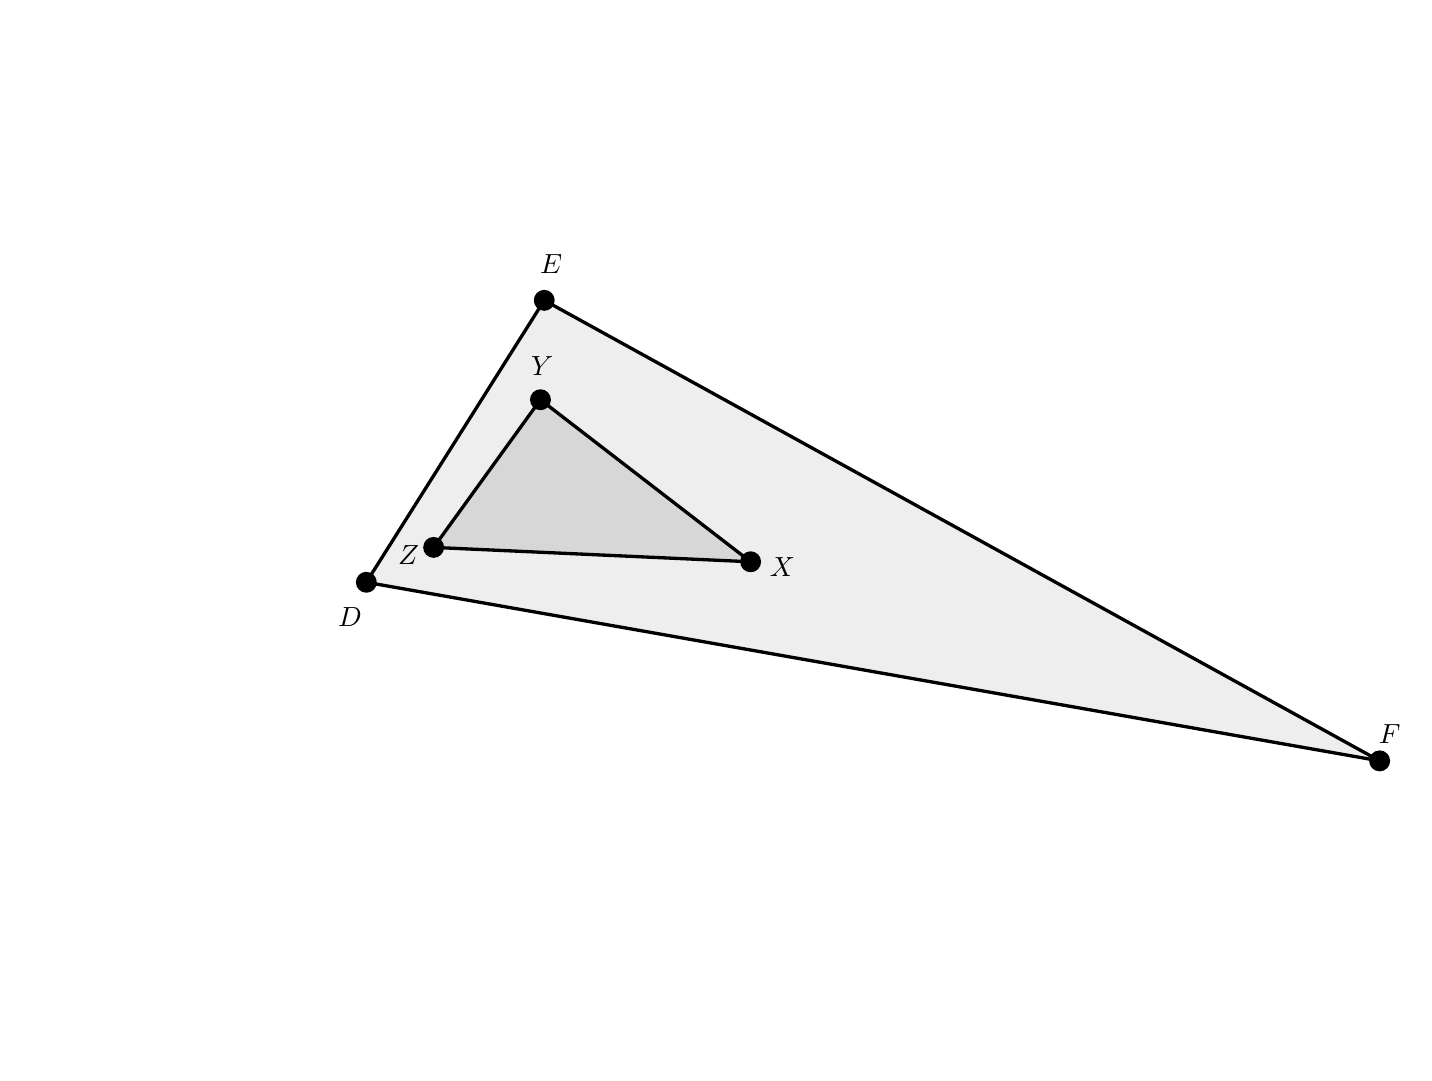
\begin{tikzpicture}[scale = 0.21]
    \clip(-29.39,-11.38) rectangle (53.84,50.63);
    \fill[line width=0pt,color=ttqqff,fill=ttqqff,fill opacity=0.15] (14.33,18.33) -- (1.62,28.13) -- (-4.84,19.2) -- cycle;
    \fill[line width=0pt,color=ttqqff,fill=ttqqff,fill opacity=0.1] (-8.91,17.09) -- (1.85,34.14) -- (52.37,6.29) -- cycle;
    \draw [line width=1.2pt] (14.33,18.33)-- (1.62,28.13);
    \draw [line width=1.2pt] (1.62,28.13)-- (-4.84,19.2);
    \draw [line width=1.2pt] (-4.84,19.2)-- (14.33,18.33);
    \draw [line width=1.2pt] (-8.91,17.09)-- (1.85,34.14);
    \draw [line width=1.2pt] (1.85,34.14)-- (52.37,6.29);
    \draw [line width=1.2pt] (52.37,6.29)-- (-8.91,17.09);
    \begin{scriptsize}
        \normalsize
        \fill [color=black] (1.62,28.13) circle (18pt);
        \draw[color=black] (1.73,30.18) node {$Y$};
        \fill [color=black] (-4.84,19.2) circle (18pt);
        \draw[color=black] (-6.35,18.76) node {$Z$};
        \fill [color=black] (14.33,18.33) circle (18pt);
        \draw[color=black] (16.26,18.01) node {$X$};
        \fill [color=black] (-8.91,17.09) circle (18pt);
        \draw[color=black] (-9.9,15) node {$D$};
        \fill [color=black] (1.85,34.14) circle (18pt);
        \draw[color=black] (2.27,36.31) node {$E$};
        \fill [color=black] (52.37,6.29) circle (18pt);
        \draw[color=black] (52.98,7.89) node {$F$};
    \end{scriptsize}
\end{tikzpicture}